\documentclass[12pt]{article}

\usepackage{amsmath, amsthm, amssymb}
\usepackage{enumitem}
\usepackage[margin=2.5cm]{geometry}
\usepackage{setspace}
\usepackage{graphicx}
\graphicspath{ {./images/} }
\usepackage{pdfpages}

\renewcommand{\baselinestretch}{1.5}
\everymath{\displaystyle}

\begin{document}
	\section*{Q3}
	\subsection*{Option 1}
	a) different k values and the accuracy:\\
	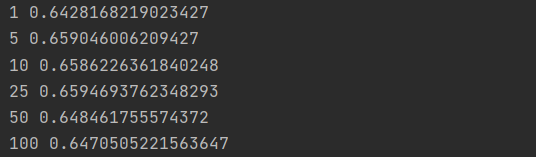
\includegraphics[scale=0.8]{a31}\\
	Take $k=25$, which gives best validation result, the final validation and test performance:\\
	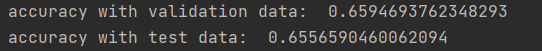
\includegraphics[scale=0.8]{a31(2)}\\
	b) SVD is filling missing entries, so it's using data that actually does not exist for prediction, which can make the results inaccurate.\\
	c) see code\\
	d) $num\_iteration=50000,\;lr=0.1$ is the chosen hyperparameters. It provides good results and convergence rate is not too slow. Different k values and accuracy:\\
	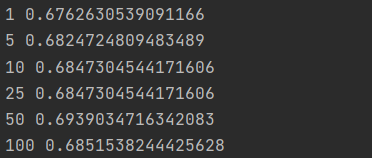
\includegraphics[scale=0.8]{a33}\\
	Take $k=50$, which gives best validation result.\\
	e) Training and validation squared-error-losses\\
	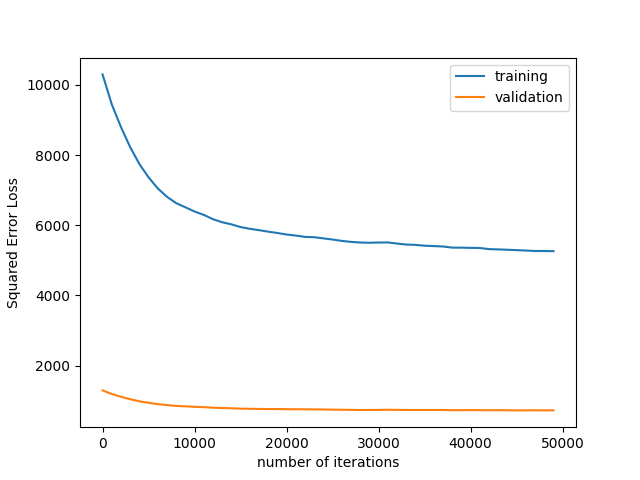
\includegraphics[scale=0.5]{a35}\\
	The final validation accuracy is $0.691645$, the final test accuracy is $0.688117$
	\newpage
	\section*{Q4}
	We would like to see if bagging improve performance of matrix factorization. So we generate 3 training data with size being the same as the original training data. We also use the same hyperparameter as in Q3 to see if there is an improvement in the accuracy with all other settings being the same. Since matrix factorization predicts with real valued probabilities, we can directly average the result to get averaged prediction of the models.\\
	Accuracy of validation data: $0.679274$; accuracy of test data: $0.679744$. Comparing to the result from Q3, there is no sign of better performance with ensemble. This is probably because ensemble reduces overfitting, and overfitting is not happening in this setting. So bagging does not improve performance.
	
	\newpage
	\section*{Part B}
	\section*{1}
	We decided to make two improvements to our model.\\
	First, we observe that the base model is treating all the questions as the same. In other word, the model believes all question reflect same level of understanding on a topic, which is unlikely to be true in reality. We believe some questions are more reflective than others on how a student understands the question. For example, if most people answer a question correctly, we believe the prediction power of this question on whether the user understand the material is quite weak. If most people answer a question wrongly, the prediction power of that question is also quite weak.\\
	So we decide to apply a weight to each question for each correct value. This should help improve the optimization. If the question is weak on prediction power, it has less weight during our calculation.\\
	We calculated the average correctness of all questions, which is about $0.6$, so we choose $0.6$ as the base. If the correctness of a question deviates a lot from $0.6$, we consider it not having enough prediction power.\\
	Another thing we add is two regularization term in the cost function. This is because after we add the weight the model becomes more important, and we want to add some regularization term to prevent it from overfitting. From our research online, these two terms are quite common for ALS model, so we choose this.\\
	Now our cost function becomes:
	\[\min_{U,Z}\frac{1}{2}\sum_{(n,m)\in O}(C_{nm}\cdot w_{m}-u_n^\top z_m)^2+\frac{1}{2}]\lambda(||u_n||^2+||z_m||^2)\]
	And the gradient descent becomes:
	\[u=u+lr(c\cdot w-u\cdot z)\cdot z+\lambda ||u||\]
	\[z=z+lr(c\cdot w-u\cdot z)\cdot u+\lambda ||z||\]
	
	\section*{2}
	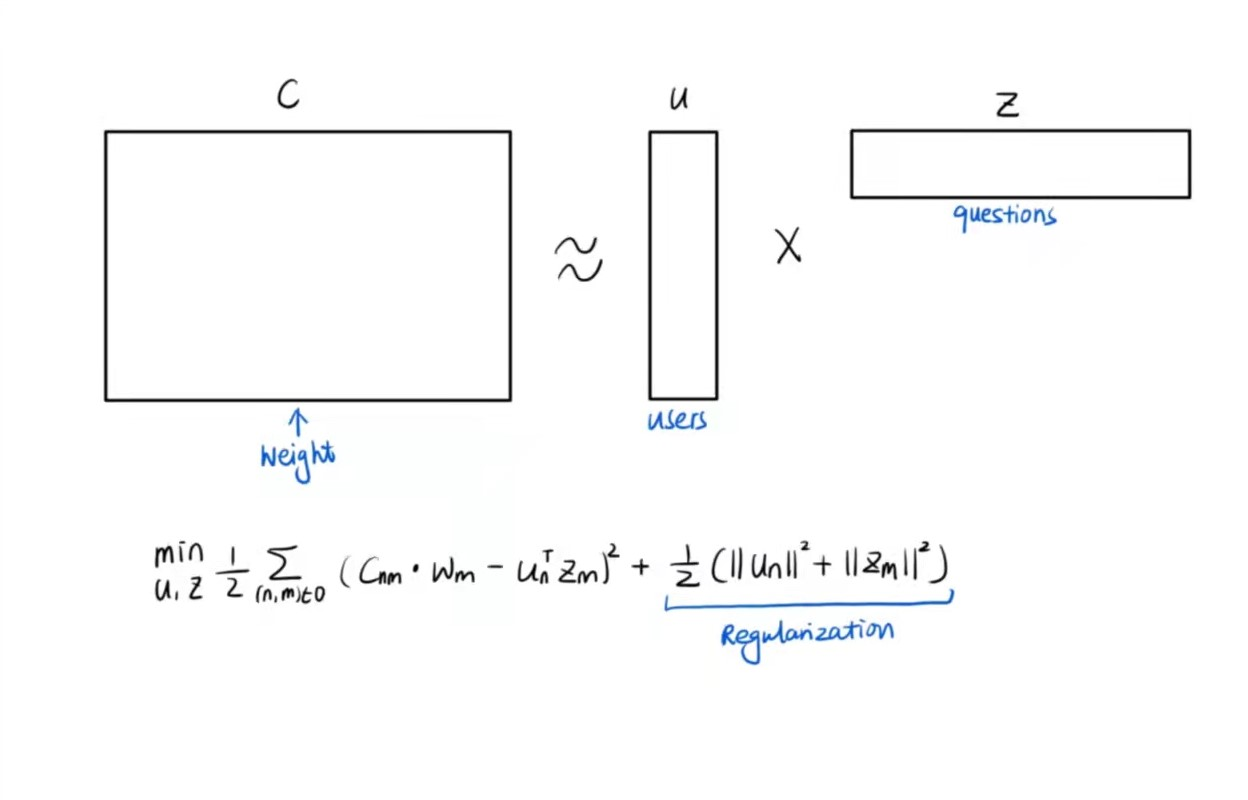
\includegraphics[scale=0.5]{b2}
	
	\section*{3}
	After experimenting with a few hyper-parameters, our accuracy on validation set and test set are as followed. The hyperparaters used are $k=50,lr=0.1, \lambda=0.01, num\_iteration=50000$. (results can vary with same input)\\
	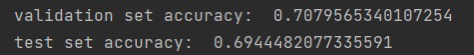
\includegraphics[scale=1]{b31}\\
	The final validation accuracy and test set accuracy of our new model are almost the same as the baseline model, which has $0.691645$ validation accuracy and $0.688117$ test accuracy.\\
	We compare the performance of the models using different values of k. The results for validation data and test data are as followed.\\
	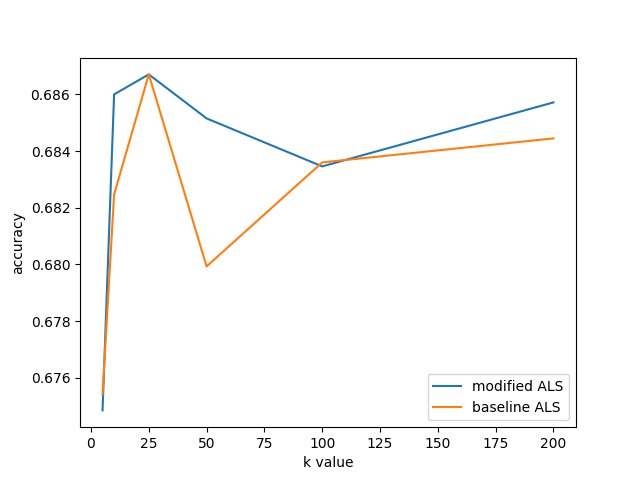
\includegraphics[scale=0.5]{b32(2)} 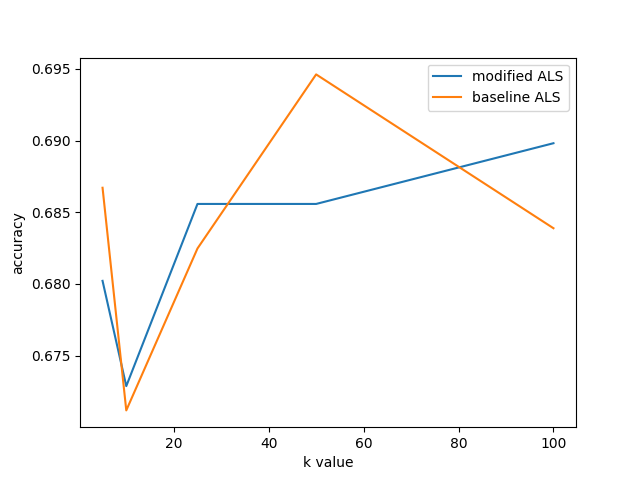
\includegraphics[scale=0.5]{b33c}\\	
	It seems the accuracy is not improved by introducing the weights and regularization term. Probably because our weights do not reflect the prediction power of data points precisely, so optimization is not improved. More factors need to be taken into account for better performance. Also we're punishing the correct answers for outlier questions only, but the wrong answer data point still have value $0$. And regularization term does not seem to have an effect on the result because the baseline model is not affected by over-fitting. So even if the regularization do reduce overfitting, we can't see this by comparing results from the two model. From this perspective, since this model is more complicated but have similar result as the base model, we can say the regularization term does prevent over-fitting.\\
	Other than the performance, we do have an improvement on running speed. The regularization term in the cost function helps the convergence process faster. It's using less time than the older version\\
	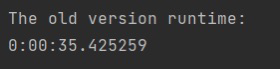
\includegraphics[scale=1]{b33a}\quad\quad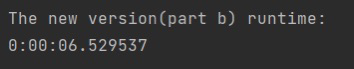
\includegraphics[scale=1]{b33b}\\
	
	
	\section*{4}
	\subsubsection*{Limitation 1}
	When we apply weight improvement to our data, we consider difficulty of the question the only factor affecting the "prediction power" of answers to that question. But this may not be the case in reality. There are other factors affecting usefulness of data point, for example, users may generate answers that do not reflect their understand of the concept by guessing.\\
	\textbf{Possible extension}: evaluate the difficulty of each question, if a user gives wrong answer to an easy question but gives correct answer to a hard question, then we punish the second data point by adding a weight to it.\\
	\subsubsection*{Limitation 2}
	When we apply weight improvement to our data, we assume the difficulty of each question are independent and follow a normal distribution. But this may not be the case in reality. If several questions are testing on related concepts, then the answers should somehow be related to each other. Also difficulties of the questions may not follow normal distribution.\\
	\textbf{Possible extension}: we can test more distribution to find the best distribution for our model.
	
	\newpage
	\section*{Reference}
	\textit
	Meira, Dania \& Viterbo, Jose \& Bernardini, Flavia. (2018). \textit{An Experimental Analysis on Scalable Implementations of the Alternating Least Squares Algorithm}. 351-359.
	
\end{document}
